\documentclass[twoside]{thesis_style/upmthesis}
\usepackage{appendix}
\usepackage{listings}
\usepackage{tabularx}
\usepackage{nameref}
\usepackage{amsmath, amssymb, latexsym}
\usepackage{graphics,epsfig,epsf,rotating,subfigure}
\usepackage{theorem,url}
\usepackage{rotfloat,array,pifont}
\usepackage{float}
\usepackage{url}
\usepackage[breaklinks]{hyperref}
\usepackage[table,usenames,dvipsnames]{xcolor}
\usepackage{dblfloatfix}
\usepackage{array}
\usepackage[T1]{fontenc}
\usepackage{clipboard}
\usepackage{amssymb}% http://ctan.org/pkg/amssymb
\usepackage{pifont}% http://ctan.org/pkg/pifont
\newcommand{\cmark}{\ding{51}}%
\newcommand{\xmark}{\ding{55}}%
% \usepackage[default,scale=0.8]{helvetica}
\usepackage[font=small,labelfont=bf]{caption}
\usepackage{fancyhdr,lipsum}
%\usepackage{emptypage} % To remove headers and page numbers from empty pages
\usepackage[all]{nowidow}

\usepackage{acronym}

\usepackage{lscape}
\usepackage[perpage]{footmisc}
%\usepackage[spanish]{babel}
\usepackage{color}

\usepackage{xspace}
\definecolor{lightgray}{rgb}{.9,.9,.9}
\definecolor{darkgray}{rgb}{.2,.2,.2}
\definecolor{purple}{rgb}{0.65, 0.12, 0.82}
\definecolor{mediumgrey}{rgb}{0.4, 0.4, 0.4}
\definecolor{etsit_orange}{rgb}{1, 0.58, 0}
\usepackage{graphicx}
\usepackage{multirow}
\usepackage{chngcntr}
\usepackage{textcomp}
\usepackage{enumitem}
\usepackage{tabu}
\usepackage{float}
\usepackage{bm}
%\usepackage[normalem]{ulem}
\counterwithout{figure}{chapter}
\counterwithout{table}{chapter}
\usepackage[noadjust]{cite}
\newcolumntype{x}[1]{>{\centering\arraybackslash\hspace{0pt}}p{#1}}
\newcolumntype{C}[1]{>{\centering\arraybackslash}p{#1}}
\newcolumntype{L}[1]{>{\arraybackslash}p{#1}}
 
\usepackage[utf8]{inputenc}
%\usepackage{tabu}
%\usepackage{hyperref}
\hypersetup{
    colorlinks,
    citecolor=black,
    filecolor=black,
    linkcolor=black,
    urlcolor=black,
    linktoc=all
}
\usepackage{xpatch}

\usepackage{refcount}
\usepackage{calc}
\newcommand{\numitemssum}[2]{\getrefnumber{#1}+\getrefnumber{#2}}


\newcommand{\numitems}[1]{\getrefnumber{#1}}
\newcounter{itemcntr}

\AtBeginEnvironment{itemize}{%
\setcounter{itemcntr}{0}%
\xapptocmd{\item}{\refstepcounter{itemcntr}}{}{}%
}
%% Customize the header and footer
\fancypagestyle{plain}{%
    \fancyhf{}{} % clear all header and footer fields
    \fancyhead[LE]{\color{black}\footnotesize\rightmark}
    \fancyhead[RO]{\color{black}\footnotesize\leftmark}
    %\fancyfoot[RO,LE]{\color{black}\footnotesize\thepage}
    \fancyfoot[C]{\color{black}\footnotesize\thepage}
    
    \renewcommand{\footrulewidth}{0pt}
    \renewcommand{\headrulewidth}{0pt}
}
% Customize the empty page between chapters so it has no header and footer (only page number)
\fancypagestyle{inbetween}{%
    \fancyhf{}{} % clear all header and footer fields
    \fancyfoot[C]{\color{black}\footnotesize\thepage}
    \renewcommand{\footrulewidth}{0pt}
    \renewcommand{\headrulewidth}{0pt}
}

\makeatletter
\def\cleardoublepage{\clearpage\if@twoside \ifodd\c@page\else
   \hbox{}\thispagestyle{inbetween}\newpage\if@twocolumn\hbox{}\newpage\fi\fi\fi}
\makeatother

\pagestyle{plain}
 

\title{Título de la tesis}

\author{Nombre completo del alumno}{Ingeniero de Telecomunicación}
\director{Nombre completo del director 1}{Doctor Ingeniero de Telecomunicación}
 \codirector{Nombre completo del director 2}{Doctor Ingeniero de Telecomunicación}
\donedatefront{22}{February}{2021} 

\committeedate{\rule{1cm}{0.15mm}}{\rule{2cm}{0.15mm}}{\rule{1.5cm}{0.15mm}} 

\university{Universidad Politécnica de Madrid}
\school{Escuela Técnica Superior de Ingenieros de Telecomunicación}
\department{Departamento de Ingeniería de Sistemas Telemáticos}
\degree{Tesis doctoral}
\addr{Madrid}{España}

\committeepresident{\hrulefill}
\committeesecretary{\hrulefill}
\committeevocala{\hrulefill}
\committeevocalb{\hrulefill}
\committeevocalc{\hrulefill}
\committeesubstitutea{\hrulefill}
\committeesubstituteb{\hrulefill}

\tolerance=1
\emergencystretch=\maxdimen
\hyphenpenalty=10000
\hbadness=10000
\vbadness=10000
\setlength{\parindent}{3em}
\setlength{\parskip}{1em}
\makeindex

\counterwithin{figure}{chapter}
\counterwithin{table}{chapter}

\begin{document}

\makefrontmatter{content/abstract}{content/ack}{content/acronyms}
\setlength{\parindent}{3em}
\setlength{\parskip}{1em}
\setlength{\baselineskip}{2em}


\raggedbottom
\setcounter{secnumdepth}{3}
\chapter{Introduction}
\label{chapter:intro}

Introduction of the thesis. Sample citation \cite{comparing}. Sample acronym: \ac{UPM} 



The present thesis aims to contribute to the growing field of *** by answering the following \acp{RQ}:
 
\begin{enumerate}
    \item \label{rq:one} \textit{\Copy{rqone}{What is my first research question?}}
    \item \label{rq:two} \textit{\Copy{rqtwo}{What is my second research question?}}
\end{enumerate}



\section{Objectives}

The main aim of this thesis is to contribute to the understanding of ****. In order to make the aforementioned contributions, the following objectives have been formulated:

\begin{enumerate}
    \item \label{obj:one} \textit{\Copy{objone}{Objective 1 of the thesis.}}
    
    \item \label{obj:two} \textit{\Copy{objtwo}{Objective 2 of the thesis}}
    
    
\end{enumerate}

Lastly, based on the achievement of these objectives, this thesis aims to answer the research questions previously stated.

\section{Research methodology}

This section describes the methodology followed in this thesis in order to achieve the specific goals previously stated and answer the research questions.

\section{Structure of this document}

\noindent \textbf{Chapter \ref{chapter:rw}: \nameref{chapter:rw}}

\vspace{-3mm}
\noindent This chapter provides an introduction to the field of ***. Objective \ref{obj:one} of this thesis is addressed in this chapter. In addition, \acp{RQ} \ref{rq:one} is answered in this chapter.
 
\noindent \textbf{Chapter \ref{chapter:something}: \nameref{chapter:something}}

\vspace{-3mm}
\noindent  This chapter reports on  Objective \ref{obj:two} and  \ac{RQ} \ref{rq:two} are addressed in this chapter. 

...

\noindent \textbf{Chapter \ref{chapter:validation}: \nameref{chapter:validation}}

\vspace{-3.5mm}
\noindent This chapter briefly describes the projects and learning experiences through which the contributions of this thesis have been validated, and lists the different publications that have been produced as a result of it. Furthermore, this chapter exhibits the contribution of this thesis to the research and educational communities through open-source software.


\noindent \textbf{Chapter \ref{chapter:conclusions}: \nameref{chapter:conclusions}}

\vspace{-3.5mm}
\noindent This chapter concludes the thesis with a summary of the answers to the research questions, a synthesis of the main contributions and some suggestions for further research. \noclub
\chapter{State of the art}
\label{chapter:rw}

\chapter{Title of this chapter}
\label{chapter:something}


Abstract of chapter 1

\section{Introduction}


\section{Objectives}
\label{section:ch03:objectives}

This chapter addresses the following objective of the thesis:

\begin{itemize}
    \item \textit{\Paste{objtwo}}

\end{itemize}


This chapter also covers the following research question:

\begin{itemize}
    \item \textit{\Paste{rqtwo}}
\end{itemize}

This question is answered based on ....

\section{Methods}

\begin{figure}[H]
\centering
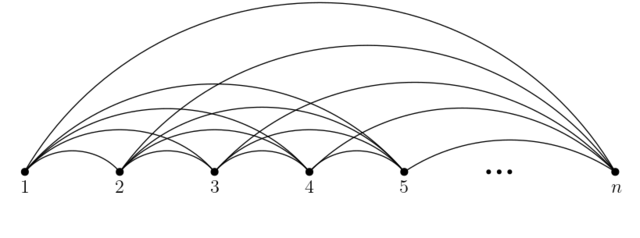
\includegraphics[width=\textwidth]{figures/sample_graph.png}
\caption{Figure caption goes here}

\end{figure}

Example code excerpt
\begin{lstlisting} 
Name.prototype = {
  methodName: function(params){
    var doubleQuoteString = "some text";
    var singleQuoteString = 'some more text';
    // this is a comment
    if(this.confirmed != null && typeof(this.confirmed) == Boolean){
      document.createElement('h3');
      $('#system').append("This looks great");
      return false;
    } else {
      throw new Error;
    }
  }
}
\end{lstlisting}


\chapter{Validation and Results}
\label{chapter:validation}
\newcommand{\Sum} [4] {\the\numexpr #1 + #2 + #3 + #4 + 1 \relax}
\def \totalPubs {\Sum{\numitems{jcr:last}}{ \numitems{sjr:last}}{\numitems{conf:last}}{\numitems{confnat:last}}}

This thesis makes several contributions to .... This chapter briefly describes the projects and learning experiences through which these contributions have been validated and lists the \totalPubs{} publications that have been produced as a result of this thesis. These publications include \numitems{jcr:last} articles in journals indexed in the \ac{JCR}, \numitems{sjr:last} article in a journal indexed in the \ac{SJR}, \numitems{conf:last} international conference papers, and \numitems{confnat:last} national conference papers. Finally, this chapter also provides a brief description of this project and some minor open source projects that have been derived from it.

This chapter is arranged as follows. In Section \ref{ch07:projects}, the projects in which several contributions of this thesis have been validated are described. Section \ref{ch07:le} reports the learning experiences in which the educational escape rooms examined in this thesis have been conducted. Section \ref{ch07:pubs} lists the publications produced as a result of this thesis. Lastly, Section \ref{ch07:os} offers a brief description of the contributions of this thesis to the open source community. 

\section{Projects}
\label{ch07:projects}
...


\section{Learning experiences}
\label{ch07:le}
...


\section{Publications}
\label{ch07:pubs}
This section lists the \totalPubs{}  publications produced as a direct or indirect result of the work conducted to develop this thesis. These publications include \numitems{jcr:last} articles in journals indexed in the \ac{JCR}, \numitems{sjr:last} article in a journal indexed in the \ac{SJR}, \numitems{conf:last} international conference papers, \numitems{confnat:last} national conference papers, and a teacher's guide distributed through an official digital repository of \ac{UPM}. 

\paragraph{Articles in international journals indexed in the JCR}

\begin{itemize}
   \small
  \item \textbf{S. López-Pernas}, A. Gordillo, E. Barra, and J. Quemada, ``Comparing Face-to-Face and Remote Educational Escape Rooms for Learning Programming,'' \textit{IEEE Access}, vol. 9, pp. 59270-59285, 2021. \\ \textbf{Impact factor:} 3.745 (JCR 2019, Q1)
\end{itemize}

\newpage
\paragraph{Articles in international journals indexed in the SJR}

...
\paragraph{International Conference Papers}

...

\paragraph{National Conference Papers}

...

\paragraph{Other}

...




\section{Open source projects}
\label{ch07:os}

\chapter{Conclusions}
\label{chapter:conclusions}


This chapter concludes this thesis with a summary of the answers to the research questions, a recapitulation of the main contributions, and some suggestions for further research. The chapter is structured as follows. The first section provides a summary of the answers to the research questions of this thesis, which were stated in Chapter \ref{chapter:intro} and answered in detail throughout the subsequent chapters. The section after that summarizes the main contributions made by this thesis to **** Lastly, the last section of this chapter provides some proposals for future research on the growing field of ****.
\newpage

\section{Research questions}

\paragraph*{Research Question \ref{rq:one}: \Paste{rqone}}\mbox{}

 
\noindent  This question can be answered based on the literature review presented in Chapter \ref{chapter:rw}, which analyzes the current approaches to ***.


\newpage
\paragraph*{Research Question \ref{rq:two}: \Paste{rqtwo}}\mbox{}

\noindent  This question can be answered based on the literature review presented in Chapter \ref{chapter:something},...


\newpage
\section{Main contributions}

The main contribution of this thesis is ***


The first contribution of this thesis is the review of the existing literature on  *** reported in Chapter \ref{chapter:rw}, which examines ***

The remaining of the present section summarizes the main contributions of this thesis to ****

\subsection{Contribution to the ****}

This thesis makes several contributions to the ***



\subsection{Contribution to the***}

This thesis makes a substantial contribution to the***


\section{Future work}

This thesis addresses many open questions and challenges in the field of ***. In this section, some proposals of interesting directions for future research on ***** are presented.




%%%%%%%%%%%%%%%%%

% UNCOMMENT NEXT LINES FOR APPENDICES
%\appendix
%\renewcommand\chaptername{Appendix}  
%\renewcommand{\thechapter}{\Roman{chapter}}
%\noappendicestocpagenum
%\appendixpage
%\addappheadtotoc
%\chapter{Análisis de Impacto}
%\include{content/append-a}
% \addcontentsline{toc} {chapter}{\numberline {}Appendix A}
%%%%%%%%%%%%%%%%%
\bibliographystyle{ieeetr}  
\bibliography{thesis}
\addcontentsline{toc} {chapter}{Bibliography}{}

\end{document} 
